% 9-17(9쪽) — 두 함수 y=f(x)(왼쪽) · y=g(x)(오른쪽) 의 그래프를 나란히. 스캔 화질이 낮아 TikZ 로 다시 그림.
% 원문에 있는 것만: f 의 눈금 −1 1 2 (x) · 2 1 −1 (y), g 의 눈금 −1 (x 축 위) · 1 (x) · 1 (y) · 라벨 O, x, y, y=f(x), y=g(x) · 좌표 안내 파선.
% 오른쪽 그래프는 같은 그림 안에서 원문의 두 좌표평면 간격(7.4칸 = 5.18cm)만큼 옮겨 그린다.
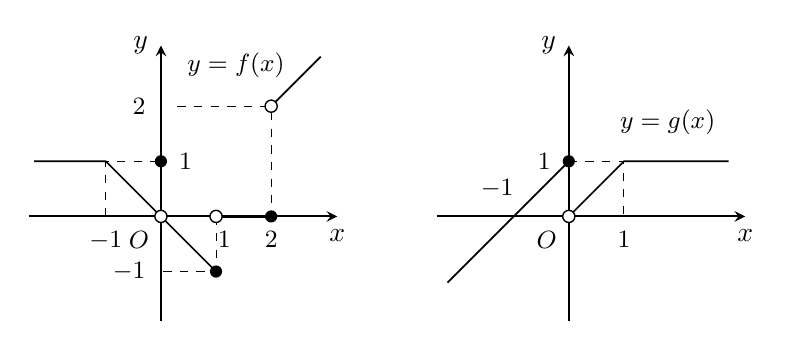
\begin{tikzpicture}[x=0.70cm, y=0.70cm, line width=0.5pt]
  % ── 왼쪽: y=f(x)
  \draw[->, >=stealth, line width=0.7pt] (-2.4,0) -- (3.2,0) node[below=1pt] {$x$};
  \draw[->, >=stealth, line width=0.7pt] (0,-1.9) -- (0,3.1) node[left=1pt] {$y$};
  \node[below=2pt, font=\small] at (-0.4,0) {$\pt{O}$};
  \draw[dashed, line width=0.35pt] (-1,0) -- (-1,1) -- (0,1);
  \draw[dashed, line width=0.35pt] (0.3,2) -- (2,2) -- (2,0);
  \draw[dashed, line width=0.35pt] (1,0) -- (1,-1) -- (0,-1);
  \draw[line width=0.6pt] (-2.3,1) -- (-1,1) -- (1,-1);
  % 이 조각은 x축 위에 그대로 놓이므로 축(0.7pt)보다 굵게 그려야 원문처럼 그래프로 보인다.
  \draw[line width=1.1pt] (1,0) -- (2,0);
  \draw[line width=0.6pt] (2,2) -- (2.9,2.9);
  \fill (0,1) circle (2.2pt);
  \fill (1,-1) circle (2.2pt);
  \fill (2,0) circle (2.2pt);
  \draw[fill=white, line width=0.5pt] (0,0) circle (2.2pt);
  \draw[fill=white, line width=0.5pt] (1,0) circle (2.2pt);
  \draw[fill=white, line width=0.5pt] (2,2) circle (2.2pt);
  \node[left=2pt, font=\small] at (0,2) {$2$};
  \node[right=3pt, font=\small] at (0,1) {$1$};
  \node[left=2pt, font=\small] at (0,-1) {$-1$};
  \node[below=2pt, font=\small] at (-1,0) {$-1$};
  \node[below=2pt, font=\small] at (1.15,0) {$1$};
  \node[below=2pt, font=\small] at (2,0) {$2$};
  \node[right=1pt, font=\small] at (0.25,2.75) {$y=f(x)$};
  % ── 오른쪽: y=g(x)
  \begin{scope}[xshift=5.18cm]
    \draw[->, >=stealth, line width=0.7pt] (-2.4,0) -- (3.2,0) node[below=1pt] {$x$};
    \draw[->, >=stealth, line width=0.7pt] (0,-1.9) -- (0,3.1) node[left=1pt] {$y$};
    \node[below=2pt, font=\small] at (-0.4,0) {$\pt{O}$};
    \draw[dashed, line width=0.35pt] (0,1) -- (1,1) -- (1,0);
    \draw[line width=0.6pt] (-2.2,-1.2) -- (0,1);
    \draw[line width=0.6pt] (0,0) -- (1,1) -- (2.9,1);
    \fill (0,1) circle (2.2pt);
    \draw[fill=white, line width=0.5pt] (0,0) circle (2.2pt);
    \node[left=3pt, font=\small] at (0,1) {$1$};
    \node[above=2pt, font=\small] at (-1.3,0.05) {$-1$};
    \node[below=2pt, font=\small] at (1,0) {$1$};
    \node[right=1pt, font=\small] at (0.7,1.7) {$y=g(x)$};
  \end{scope}
\end{tikzpicture}
